% Chapter 5

\chapter{安全性设计}

\section{生成安全的前端页面}

所有返回给用户的前端页面都经由Thymeleaf模板引擎渲染而成,我们遵照规范,正确的使用了Thymeleaf模板,因此从源头杜绝了所有可能的XSS攻击,包括Stored XSS和Reflected XSS漏洞都不会出现在我们的网站中。下面是一个典型的Thymeleaf模板示例。

\begin{minted}
[
	frame=lines,
	framesep=2mm,
	baselinestretch=1.2,
	bgcolor=lightgray,
	fontsize=\footnotesize,
	linenos
]{html}

<div class="w3-card-4 w3-padding-16 w3-white w3-container" th:if="${has_error}">
     <div class="w3-center">
            <b style="color:red" th:text="${error_msg}"></b>
     </div>
</div>

\end{minted}

\vspace{-3ex}
\begin{algorithm}[H]
  \caption{Thymeleaf模板}
\end{algorithm}

\section{校验用户输入}

任何由用户提交给服务器端的信息都有可能成为恶意攻击者的突破口,忽视或不完善的校验检查往往会让恶意攻击者有机可乘。我们对所有用户输入都做了严格的校验检查,并且是前端和后端的双重检查。

\subsection{注册表单校验规则}\label{sec:registerV}

\begin{itemize}
	\item \textbf{用户名校验规则}
	
	为保证用户名的强度,我们要求一个合法的用户名必须不少于6个字符,并不多于18个字符。每一个字符都必须是ASCII字母,ASCII数字,或者下划线“\_”。
	
	\item \textbf{密码校验规则}
	
	密码的强度对于一个系统的安全来说至关重要,弱密码如“123456”、“root”、“qwert”都极易被攻击者猜中。因此为保证用户的密码强度,我们要求一个合法的密码必须必须不少于6个字符,并不多于18个字符。每一个字符都必须是可打印出来的ASCII字符。并且整个密码必须同时包含大写字母、小写字母、数字和特殊符号(例如百分号、下划线等)。
	
	\item \textbf{电子邮箱地址校验规则}
	
	我们认为电子邮箱地址应当是一个合法的互联网地址,因此利用了JavaMail中的InternetAddress类来校验它。代码示例如下。
	
\begin{minted}
[
	frame=lines,
	framesep=2mm,
	baselinestretch=1.2,
	bgcolor=lightgray,
	fontsize=\footnotesize,
	linenos
]{java}

public static boolean isValidEmail(String email) {
        try {
                InternetAddress emailAddr = new InternetAddress(email);
                emailAddr.validate();
                return true;
        } catch (AddressException ex) {
                return false;
        }
}

\end{minted}

\vspace{-3ex}
\begin{algorithm}[H]
  \caption{验证电子邮箱地址}
\end{algorithm}
	
	\item \textbf{重复密码校验规则}
	
	为确保用户输入了其设想中的密码,避免由于键盘误操作带来的错误。我们要求用户输入两次索要设置的密码,只有两次密码完全相同的时候才被认为密码正确,通过校验。
	
\end{itemize}

\subsection{电子邮箱的验证规则}\label{sec:emailV}

用户在刚刚注册完,或者是刚刚更换电子邮箱地址之后。这个新的电子邮箱地址会处于“未验证”的状态。我们估计用户通过我们的系统验证这个电子邮箱地址。当用户在登录后点击个人主页中的“VERIFY YOUR EMAIL ADDRESS”链接后,一封电子邮件会被发送到用户指定的邮箱中,其中会包含一个链接,点击该链接就可以完成对电子邮箱的验证。

\subsection{文件上传的验证规则}\label{sec:fileV}

文件的上传在网络生活中及其常见,应用广泛。但往往不严谨的实现会留下安全隐患,给恶意攻击者留下攻击服务器的空间。我们在这里进行了多次验证,主要防范了以下的潜在攻击方式
\begin{itemize}

	\item \textbf{耗尽服务器资源的攻击}
	
	为了防止服务器的磁盘资源被恶意攻击者用很多大文件抢占一空,我们限制了单个上传的文件大小上限,现阶段我们只允许上传小于10MB的文件。
	
	\item \textbf{恶意文件名攻击}
	
	恶意攻击者有可能会上传形如“../../file.txt”的文件,使得该文件有可能会存储在服务器指定的存储根目录外,造成未知的、及其难以排查的错误。因此我们会仔细检查文件名,拒绝所有包含路径分隔符的非法文件名。同时我们再实际存储的时候会随机生成一个随机的字符串作为文件名(文件标识符),进一步降低出现漏洞的可能性。
	
	\item \textbf{恶意程序注入}
	
	恶意攻击者有可能会上传包含恶意程序的代码片段,并试图通过别的手段让这段代码在服务器端运行,从而制造后门或或获取更大的服务器权限。因此我们采取文件拓展名白名单的形式限制了可以上传的文件类型。只有形如以下拓展名的文件才能被成功上传:
	\begin{itemize}
		\item \textbf{文档类}
		
		docx,doc,pptx,ppt,xlsx,xls,pdf
		
		\item \textbf{图片类}
		
		jpeg,jpg,png,gif,tiff,tif,raw,bmp,svg
		
		\item \textbf{纯文本类}
		
		txt,tex,md
		
		\item \textbf{音频类}
		
		mp3,wav
		
		\item \textbf{压缩类}
		
		zip,z,rar,7z,gz,tar
		
		\item \textbf{数据类型}
		
		csv,xml
	\end{itemize}

\end{itemize}

\section{Session安全分析}\label{sec:sessionS}

我们为用户生成的的Cookie是长达16字节的随机数。16个字节总共会包含128个比特,即一共会有$2^{128}$种可能的排列组合。这个取值空间是如此之大,基本上可以近似于认为我们的Session是永远不会重复的,没有重用的风险。同时Session会有有效时间的限制,如果用户在30分钟内没有进行任何操作的话,用户的Session将会过期,需要重新登录。

\section{处理错误和异常}

由于未被catch的exception,或者其他种种难以预料到的情形,服务器常常会产生错误的响应。这类错误信息如果未经处理是及其危险的,因为往往默认的做法是打印stack trace(如图\ref{fig:stacktrace})。这样的暴露是及其危险的,其中很有可能会泄露部分代码细节,从而让恶意攻击者找到下一步攻击服务器的突破口,进而带来更大的恶劣影响。在本项目中,我们统一编写了一个用于在异常情况下响应的控制器,该控制器会返回我们自己设计的统一风格的错误界面,在保证整体网站风格统一的前提下,隐藏了所有可能会暴露代码细节的信息。

\begin{figure}[!htb]
	\centering
	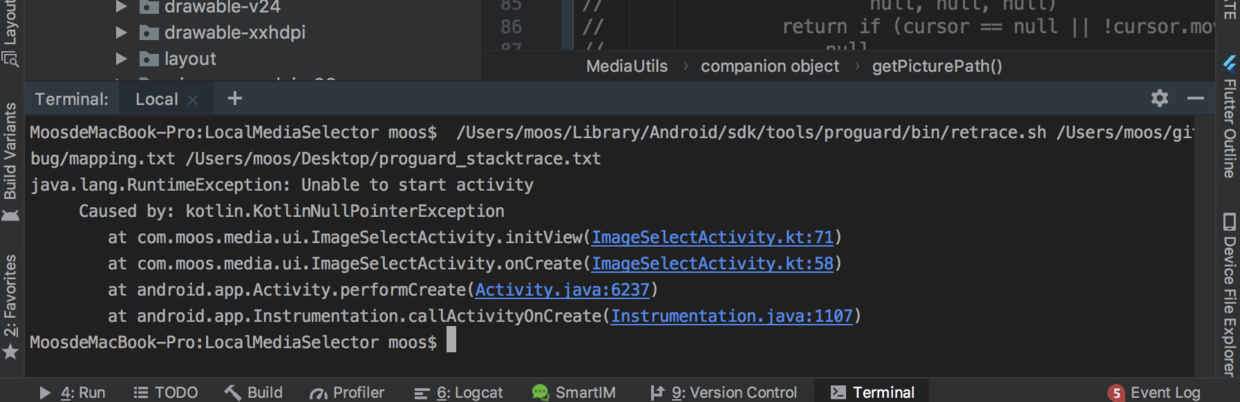
\includegraphics[width=0.8\textwidth]
	{figures/stacktrace.jpg}\\
	\caption{可能会暴露代码细节信息的stack trace}
	\label{fig:stacktrace}
\end{figure}

\section{存储哈希过后的密码}\label{sec:hashpassword}

为了让用户能够登陆我们的系统,我们势必需要在后台数据库中存储下用户的密码信息,取决于存储的方案,用户密码的安全性会有很大的区别。

如果直接明文存储用户的密码信息,一旦服务器端的数据泄露,用户所有的密码信息都会造成不可挽回的全面泄露,这样的安全性是不可接受的。

一个可行的改进方案是存储密码的散列哈希数值,而非密码明文本身。由于散列哈希函数是单向的、不可逆的,因此即便服务器端的数据库遭到了整体泄露,恶意攻击者仍然不能从密码的哈希散列值反推出密码本身,显著地提高了数据库的安全性。

但这样的措施仍然留给了恶意攻击者进行离线攻击的空间。因为日常生活中用户使用的密码往往强度不高,并且有大量的密码是常见的、会被用户重复在不同平台使用的。所以恶意攻击者可以实现搜集这样的已知密码组合,构成密码字典。然后恶意攻击者事先计算出密码字典中密码的哈希散列值,然后在攻破数据库后就仅仅需要进行比对即可得知用户的原始密码明文。

为了阻止恶意攻击者进行离线攻击,一个可行的改进方案是加入盐(salt),即用户的密码会和一组被称为盐的随机数据叠加在一起然后进行哈希,盐会直接明文存储在数据库中。由于哈希函数设计的原则——输入的任何细微变化都会导致输出产生近似于随机的巨大变化——恶意攻击者必须在攻破数据库后在线重新计算其所拥有的密码字典中的哈希散列值。进而阻止一切离线字典攻击的可能。

同时,虽然我们无法从根源上阻止恶意攻击者进行在线攻击的可能性,但是我们可以增加其在线攻击的困难程度,从而间接进一步提高安全性。一个可行的做法是使用更慢的哈希算法,假设我们使用了比一般哈希算法慢1000倍的安全哈希算法。一个相同的恶意攻击者就需要花费之前1000倍的时间才能完成同样的一次在线字典攻击。

\begin{minted}
[
	frame=lines,
	framesep=2mm,
	baselinestretch=1.2,
	bgcolor=lightgray,
	fontsize=\footnotesize,
	linenos
]{java}

public static byte[] getHashedPassword(String password, byte[] salt) {
        byte[] hashedPassword = null;
        try { // PBKDF2
                KeySpec spec = new PBEKeySpec(
                        password.toCharArray(), salt, 
                        PBKDF2_ITERATION_COUNT, PBKDF2_KEY_SIZE);
                SecretKeyFactory factory = SecretKeyFactory.getInstance("PBKDF2WithHmacSHA1");
                hashedPassword = factory.generateSecret(spec).getEncoded();
        } catch (InvalidKeySpecException | NoSuchAlgorithmException e) {
                e.printStackTrace();
        }
        return hashedPassword;
}

\end{minted}

\vspace{-3ex}
\begin{algorithm}[H]
  \caption{哈希密码}
\end{algorithm}

因此我们选择将用户的密码以及随机生成盐通过PBKDF2算法进行哈希加密,然后存储于数据库中。
代码如上述代码片段所示。
作为PBKDF2的优点之一,它还可以通过调节循环哈希次数的方式调节算法的强度。
也就是说即便未来出现了计算性能1000倍于当前计算机的超级计算机,我们也仅需将重复次数增大1000倍即可获得相同的算法强度。
上述代码第6行的PBKDF2\_ITERATION\_COUNT参数就是用于调节充数次数的参数,现在我们将这个参数设定为65536,即$2^{16}$。

\section{密钥的安全分析}\label{sec:keyS}

\subsection{对称加密分析}

我们通过对称加密算法对密钥、文件等数据进行加密。它的优点是安全性高,加密速度快等。一个典型的加密过程代码如下所示,首先在第1-4行生成了随机的IV,为了确保安全,我们每次都会随机生成IV,绝不会重用IV。在第5行,我们创建了Cipher对象,这里我们使用的是AES-CBC加密模式,并且用PKCS5Padding的方式进行填充。随后在第7行完成了对称加密的过程。

\begin{minted}
[
	frame=lines,
	framesep=2mm,
	baselinestretch=1.2,
	bgcolor=lightgray,
	fontsize=\footnotesize,
	linenos
]{java}

byte[] iv = new byte[IV_SIZE];
SecureRandom random = new SecureRandom(); 
random.nextBytes(iv); // generate iv randomly
IvParameterSpec ivParameterSpec = new IvParameterSpec(iv);
Cipher cipher = Cipher.getInstance("AES/CBC/PKCS5Padding");
cipher.init(mode, key, ivParameterSpec);
byte[] encryptedData = cipher.doFinal(data);

\end{minted}

\vspace{-3ex}
\begin{algorithm}[H]
  \caption{对称加密}
\end{algorithm}

\subsection{多级密钥加密结构}

为了确保数据的安全性,需要加密的文件、密钥等敏感信息都不会明文存储在数据库中,它们都会首先被正确的加密。图\ref{fig:encrypt}展示了我们的多层加密结构。

\begin{figure}[!htb]
	\centering
	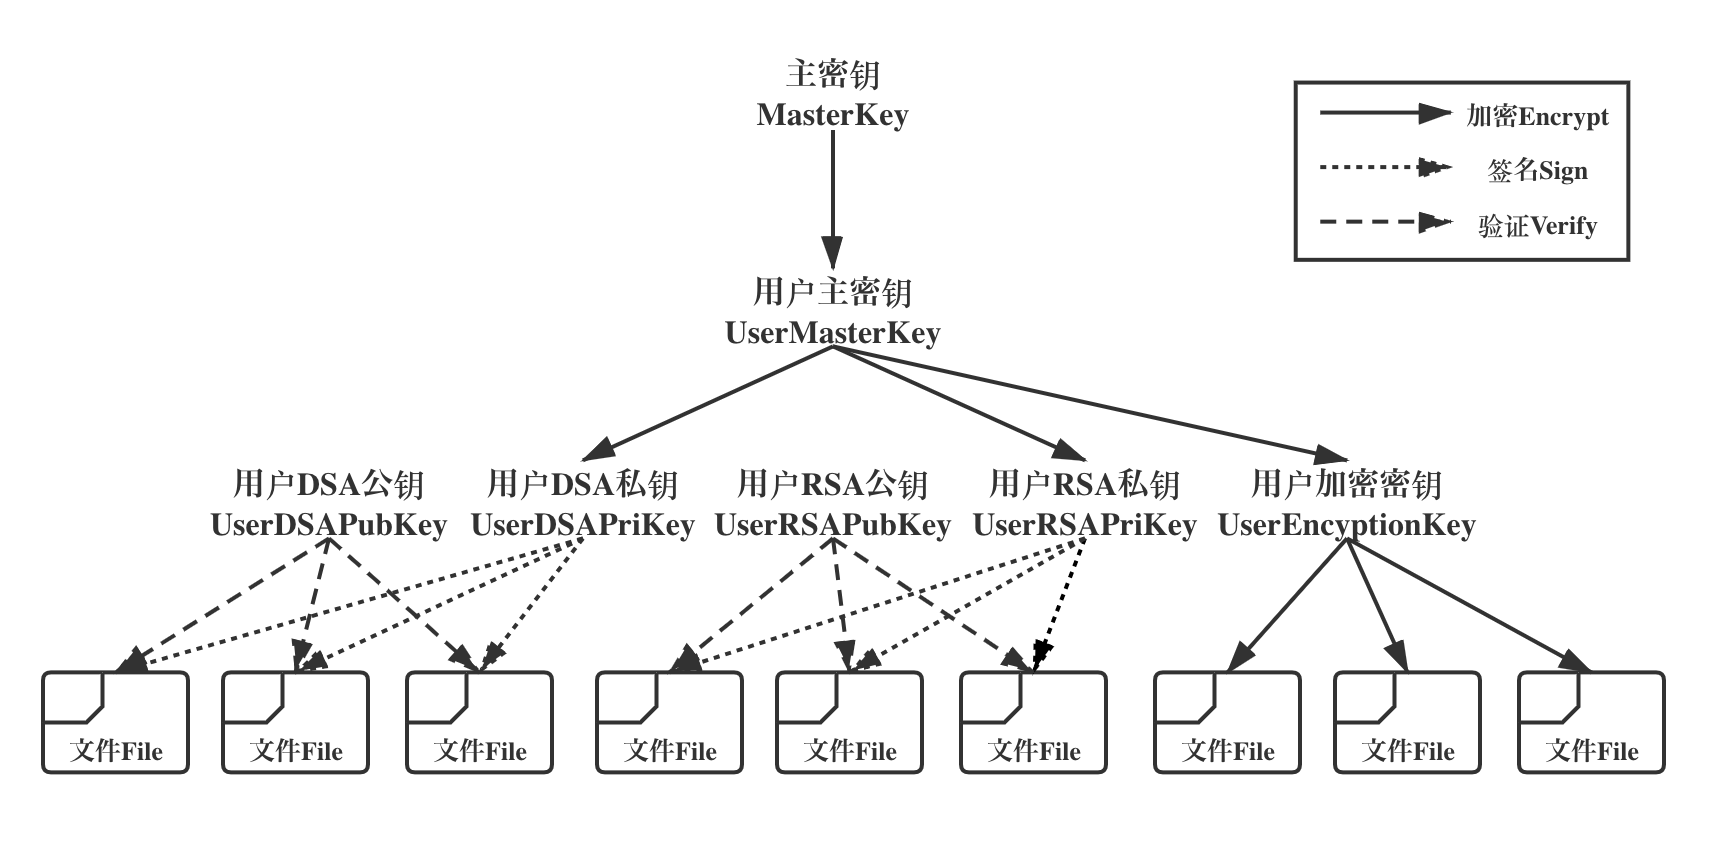
\includegraphics[width=0.8\textwidth]
	{figures/encrypt.png}\\
	\caption{多级加密结构}
	\label{fig:encrypt}
\end{figure}

位于最上端的是整个系统的主密钥,主密钥是在系统初始化的时候随机生成的,并且仅存在于内存当中。

每个用户在创建账户的时候,系统都会为其随机生成一个用户主密钥,这是第二级密钥。用户主密钥将被主密钥加密后存储于数据库中。

同时每个用户拥有自己的DSA公钥私钥对,RSA公钥私钥对和一个加密密钥。DSA公钥私钥对和RSA公钥私钥对用于对文件生成数字签名、验证数字签名。加密密钥用于加密用户指定的需要加密的文件。DSA公钥和RSA公钥不会被加密,明文存储于数据库中。DSA私钥,RSA私钥和加密密钥会被用户主密钥加密后,密文存储于数据库中。

上述所有提到的密钥都是由安全的生成器随机生成的,我们保证不会重复利用密钥。

\section{数字签名}

我们提供用DSA或者RSA算法这两种选择用于生成数字签名,一段典型的生成签名代码示例如下所示。

\begin{minted}
[
	frame=lines,
	framesep=2mm,
	baselinestretch=1.2,
	bgcolor=lightgray,
	fontsize=\footnotesize,
	linenos
]{java}

Signature signature = Signature.getInstance("SHA256WithDSA"); 
//Signature signature = Signature.getInstance("SHA256withRSA");
SecureRandom secureRandom = new SecureRandom();
signature.initSign(privateKey, secureRandom);
signature.update(data);
digitalSignature = signature.sign();

\end{minted}

\vspace{-3ex}
\begin{algorithm}[H]
  \caption{数字签名}
\end{algorithm}

第1-2行我们选择了恰当的算法,SHA256WithDSA代表先用SHA256哈希散列算法计算文件的哈希数值,然后对哈希数值用DSA算法进行签名。SHA256withRSA代表先用SHA256哈希散列算法计算文件的哈希数值,然后对哈希数值用RSA算法进行签名。

由于DSA、RSA生成的签名长度与输入数据长度有关,这样做的好处是保证我们生成的签名长度固定,同时避免对大文件进行数字签名时消耗太长的时间。